\documentclass[paper=a4, fontsize=11pt]{scrartcl} % A4 paper and 11pt font size
\usepackage{./../usfassignment}
\settitle{Assignment 7}
\setauthor{Wanzhang Sheng}
\setcourse{CS675: Automata Theory}

\begin{document}

\maketitle % Print the title

% -----------------------------------------------------------------------------
% PROBLEM 1
% -----------------------------------------------------------------------------
\section{}

\begin{fancyquotes}
   Give a diagram for a non-deterministic Turing machine that accepts
   the language $L = \{ww : w\in \{a, b\}^{*}\}$.
\end{fancyquotes}

\begin{figure}[hp]
  \centering
  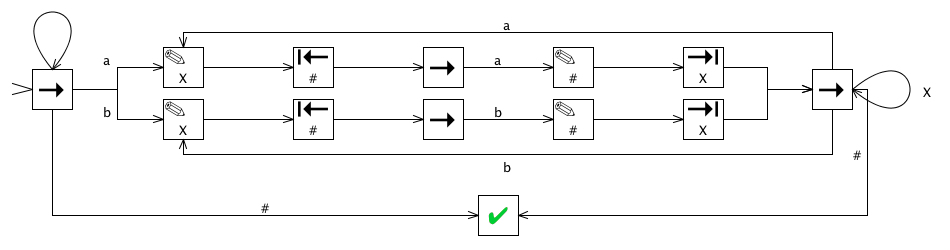
\includegraphics[width=\textwidth]{7-1.png}
  \caption{$L = \{ww : w\in \{a,b\}^{*}\}$}
\end{figure}

\pagebreak

% -----------------------------------------------------------------------------
% PROBLEM 2
% -----------------------------------------------------------------------------
\section{}

\begin{fancyquotes}
  Submited to SVN.
\end{fancyquotes}

% -----------------------------------------------------------------------------
% PROBLEM 3
% -----------------------------------------------------------------------------
\section{}

\begin{fancyquotes}
  Give an unrestricted grammar for each of the following languages:
\end{fancyquotes}

\begin{enumerate}
\item $L = \{a^{n}b^{n}c^{n}d^{n} : n\geq 0\}$.
  $$S \rightarrow ABCDS | T_d$$
  $$DA \rightarrow AD$$
  $$DB \rightarrow BD$$
  $$DC \rightarrow CD$$
  $$CA \rightarrow AC$$
  $$CB \rightarrow BC$$
  $$BA \rightarrow AB$$
  $$DT_d \rightarrow T_dd$$
  $$CT_d \rightarrow T_cc$$
  $$CT_c \rightarrow T_cc$$
  $$BT_c \rightarrow T_bb$$
  $$BT_b \rightarrow T_bb$$
  $$AT_b \rightarrow T_aa$$
  $$AT_a \rightarrow T_aa$$
  $$T_a | T_d \rightarrow \epsilon$$

\item $L = \{a^{2^{n}} : n\geq 0\}$.
  $$S \rightarrow BAE$$
  $$E \rightarrow TE$$
  $$AT \rightarrow TAA$$
  $$BT \rightarrow B$$
  $$A \rightarrow a$$
  $$B \rightarrow \epsilon$$
  $$E \rightarrow \epsilon$$

\item $L = \{a^{n^{2}} : n\geq 0\}$
  $$S \rightarrow BTE$$
  $$T \rightarrow XT | \epsilon$$
  $$X \rightarrow LYZR$$
  $$YL \rightarrow LYZ$$
  $$RY \rightarrow ZYR$$
  $$ZL \rightarrow LZ$$
  $$RZ \rightarrow ZR$$
  $$RL \rightarrow LR$$
  $$BL \rightarrow B$$
  $$RE \rightarrow E$$
  $$YE \rightarrow Ea$$
  $$ZE \rightarrow Ea$$
  $$BE \rightarrow \epsilon$$

\end{enumerate}


\pagebreak

\end{document}
